\documentclass[a4paper,12pt]{report}

\usepackage[utf8]{inputenc}
\usepackage{graphicx}
\usepackage{setspace}
\usepackage{lipsum}
\usepackage[bahasa]{babel}
\usepackage{graphicx}
\usepackage{hyperref}
\usepackage{enumitem}
\usepackage{listings}
\usepackage{xcolor}
\usepackage{tcolorbox}
\usepackage{courier}
\usepackage{fancyhdr}
\usepackage{indentfirst}
\usepackage{longtable}


% Package TikZ untuk diagram
\usepackage{tikz}
\usepackage{pgf}
\usetikzlibrary{mindmap}
\usetikzlibrary{arrows.meta}
\usetikzlibrary{positioning}
\usetikzlibrary{shapes,arrows}
\usetikzlibrary{er}
\usetikzlibrary{calc}

% Library tambahan untuk diagram kompleks
\usetikzlibrary{trees}
\usetikzlibrary{shadows}
\usetikzlibrary{backgrounds}
\usetikzlibrary{decorations}

% Atur penomoran section agar tidak terpengaruh chapter
% Ini akan memungkinkan penomoran section dimulai dari 1 di setiap chapter
\counterwithout{section}{chapter}

% Konfigurasi hyperref
\hypersetup{
    colorlinks=true,
    linkcolor=black,
    filecolor=magenta,      
    urlcolor=cyan,
    pdftitle={Modul Praktikum Sistem Manajemen Basis Data},
    pdfpagemode=FullScreen,
}

% Konfigurasi untuk kode program
\definecolor{codegreen}{rgb}{0,0.6,0}
\definecolor{codegray}{rgb}{0.5,0.5,0.5}
\definecolor{codepurple}{rgb}{0.58,0,0.82}
\definecolor{backcolour}{rgb}{0.95,0.95,0.92}

\lstdefinestyle{mystyle}{
    backgroundcolor=\color{backcolour},
    commentstyle=\color{codegreen},
    keywordstyle=\color{magenta},
    numberstyle=\tiny\color{codegray},
    stringstyle=\color{codepurple},
    basicstyle=\ttfamily\small,
    breakatwhitespace=false,
    breaklines=true,
    captionpos=b,
    keepspaces=true,
    numbers=left,
    numbersep=5pt,
    showspaces=false,
    showstringspaces=false,
    showtabs=false,
    tabsize=2
}

\lstset{style=mystyle}

% Konfigurasi header dan footer
\pagestyle{fancy}
\fancyhf{}
\fancyhead[L]{}
\fancyhead[R]{Departemen Teknik Komputer ITS}
\fancyfoot[C]{\thepage}
\renewcommand{\headrulewidth}{0.4pt}
\renewcommand{\footrulewidth}{0.4pt}

\title{Laporan Praktikum\\
Basis Data}
\author{}
\date{}


\begin{document}

% Halaman Cover
\begin{titlepage}
    \centering

    
\includegraphics[width=0.3\textwidth]{images/logo-tekkom.png}\\[1cm]

    {\Huge \textbf{Laporan Final Project}\\[0.3cm]}
    {\Huge \textbf{Machine Learning}}\\[1cm]
    
%Judul
    {\Large \textbf{Prediksi Nilai Ujian Pada Sekolah Menengah ke Atas Menggunakan Model RandomForest Regressor,XGboost,
    MLP Tensorflow,dan Linear Regresi} \\[1cm]}
%    {\Large \textbf{ke Atas Menggunakan Model RandomForest} \\[0.1cm]}
%    {\Large \textbf{Regressor,XGboost,MLP Tensorflow,dan Linear Regresi} \\[0.1cm]}

    {\Large {Muhammad Risang - 50242310xx}}\\[0.3cm]
    {\Large {Akhmad Rizqullah Ridlohi - 5024231037}}\\[0.3cm]
    {\Large {Abraham Napitupulu - 50242310xx}}\\[1cm]

    
    {\large \textit{Departemen Teknik Komputer}}\\
    {\large \textit{Institut Teknologi Sepuluh Nopember}}\\
    {\large \textit{Surabaya}}\\[0.3cm]

    \hfill Penulis: Kelompok 6\\
    \hfill 20 Juni 2025
\end{titlepage}

\tableofcontents
\clearpage



\chapter*{Dasar Teori}
\addcontentsline{toc}{chapter}{Dasar Teori}

\section{Latar Belakang dan Relevansi}
Di sistem pendidikan kita sekarang, bantuan untuk siswa yang kesulitan seringkali datang terlambat. Biasanya, sekolah baru akan bertindak---misalnya dengan mengadakan kelas remedial---setelah nilai ujian akhir keluar dan hasilnya kurang memuaskan. Tentu saja, pendekatan seperti ini punya kelemahan besar: bantuan diberikan saat semuanya sudah terjadi, di mana siswa mungkin sudah kehilangan motivasi.
Di sinilah \textit{machine learning} bisa mengubah keadaan. Dengan menganalisis data-data siswa yang sudah ada---mulai dari data pribadi, pergaulan, dan terutama nilai-nilai sebelumnya---kita bisa membuat sebuah model prediksi. Model ini bisa berfungsi seperti ``sistem peringatan dini'' yang bisa menandai siswa mana yang kemungkinan besar akan gagal, jauh sebelum ujian akhir. Dengan kemampuan ini, para guru bisa memberikan bantuan yang lebih personal dan tepat waktu, sehingga peluang siswa untuk berhasil jadi lebih besar.

\section{Tujuan dan Ruang Lingkup Proyek}
Berdasarkan masalah di atas, tujuan utama dari proyek ini adalah:
\begin{enumerate}
    \item Membuat dan melatih beberapa model \textit{machine learning} untuk memprediksi nilai akhir matematika siswa (\texttt{G3}).
    \item Membandingkan model-model tersebut untuk menemukan mana yang paling akurat dan bisa diandalkan.
    \item Menganalisis fitur atau faktor apa saja yang paling berpengaruh menurut model terbaik.
\end{enumerate}

Untuk mencapai tujuan itu, proyek ini punya batasan (ruang lingkup) sebagai berikut:
\begin{itemize}
    \item \textbf{Dataset:} Kami menggunakan dataset publik ``Student Performance'' dari UCI, yang berisi data dari 395 siswa di Portugal.
    \item \textbf{Metodologi:} Kami mengikuti alur kerja standar, mulai dari membuat fitur baru (\textit{feature engineering}), memproses data (\textit{preprocessing}), hingga melatih model.
    \item \textbf{Model yang Diuji:} Kami membandingkan beberapa jenis model: \textbf{Regresi Linear} (sebagai baseline), \textbf{Random Forest} dan \textbf{XGBoost} (sebagai model ensemble canggih), serta \textbf{Multi-Layer Perceptron (MLP)} (sebagai perwakilan deep learning).
    \item \textbf{Metrik Evaluasi:} Performa model diukur menggunakan \textbf{R-squared (R²)} dan \textbf{Root Mean Squared Error (RMSE)}.
\end{itemize}

Pendekatan untuk membandingkan berbagai model seperti ini sejalan dengan banyak penelitian di bidang \textit{Educational Data Mining}. Sebagai contoh, sebuah studi oleh Al-Barrak dan Al-Razgan (2016) juga membandingkan beberapa algoritma, termasuk \textit{Decision Trees} (yang menjadi dasar dari Random Forest dan XGBoost), untuk memprediksi IPK mahasiswa. Studi mereka juga menemukan bahwa nilai-nilai sebelumnya adalah faktor prediksi terkuat, sebuah temuan yang menjadi fondasi utama dalam analisis kami.


Dengan landasan teori ini, langkah selanjutnya adalah memahami secara mendalam dataset yang akan digunakan dalam proyek ini.

\chapter*{DataSet}
\addcontentsline{toc}{chapter}{DataSet}

\section{Deskripsi Dataset}
Dataset yang kami pilih untuk proyek ini, yaitu ``Student Performance Data Set'', lebih dari sekadar nilai-nilai tak bermakna. Ini adalah potret lengkap kehidupan para siswa. Keistimewaannya adalah data yang sangat beragam, mencakup semuanya mulai dari nilai-nilai akademik, data diri (seperti usia dan alamat), latar belakang keluarga (seperti pendidikan orang tua), hingga gaya hidup mereka (seperti waktu belajar, absensi, dan seberapa sering mereka main). Karena datanya begitu kaya dan bervariasi, ini menjadi dasar yang sempurna untuk membuat model prediksi yang bagus dan menggali faktor apa saja yang sebenarnya mengukur kesuksesan akademis seorang siswa.

\subsection{Sumber Data}
\begin{itemize}
    \item \textbf{Judul:} Student Performance Data Set
    \item \textbf{Author:} P. Cortez and A. Silva
    \item \textbf{Tanggal Terbit:} 2008
    \item \textbf{Sumber:} UCI Machine Learning Repository
    \item \textbf{Relevansi:} Dataset ini sangat relevan karena secara spesifik mencatat berbagai atribut demografis, sosial, dan akademik siswa yang dapat digunakan untuk tujuan prediksi kinerja, sejalan dengan tujuan proyek ini.
\end{itemize}

\subsection{Ukuran dan Kualitas Dataset}
\begin{itemize}
    \item \textbf{Jumlah Data:} Dataset ini terdiri dari \textbf{395 entri} (siswa).
    \item \textbf{Jumlah Fitur:} Terdapat total \textbf{33 fitur} (atribut) awal untuk setiap siswa.
    \item \textbf{Data Kosong:} Analisis awal menunjukkan bahwa dataset ini memiliki kualitas yang sangat baik, dengan \textbf{tidak ada nilai kosong} (\textit{missing values}) sama sekali, sehingga tidak memerlukan langkah mengeluarkan data.
\end{itemize}

\subsection{Fitur-fitur Relevan}
Berikut adalah deskripsi dari fitur-fitur utama yang terdapat dalam dataset:
\begin{longtable}{|p{0.15\linewidth}|p{0.15\linewidth}|p{0.6\linewidth}|}
    \caption{Deskripsi Fitur dalam Dataset} \\
    \hline
    \textbf{Nama Variabel} & \textbf{Tipe Data} & \textbf{Deskripsi} \\
    \hline
    \endfirsthead

    \hline
    \textbf{Nama Variabel} & \textbf{Tipe Data} & \textbf{Deskripsi} \\
    \hline
    \endhead

    \hline
    \endfoot

    \hline
    \endlastfoot

    school & Kategorikal & Sekolah siswa (`GP` atau `MS`) \\
    sex & Biner & Jenis kelamin siswa (`F` atau `M`) \\
    age & Integer & Usia siswa (15 hingga 22) \\
    address & Kategorikal & Tipe alamat rumah (`U` - urban atau `R` - rural) \\
    famsize & Kategorikal & Ukuran keluarga (`LE3` - ≤3 atau `GT3` - >3) \\
    Pstatus & Kategorikal & Status kohabitasi orang tua (`T` - bersama atau `A` - berpisah) \\
    Medu & Integer & Pendidikan Ibu (0 = tidak ada, 4 = pendidikan tinggi) \\
    Fedu & Integer & Pendidikan Ayah (0 = tidak ada, 4 = pendidikan tinggi) \\
    Mjob & Kategorikal & Pekerjaan Ibu (`teacher`, `health`, `services`, dll.) \\
    Fjob & Kategorikal & Pekerjaan Ayah (`teacher`, `health`, `services`, dll.) \\
    studytime & Integer & Waktu belajar mingguan (1 = <2 jam, 4 = >10 jam) \\
    failures & Integer & Jumlah kegagalan kelas sebelumnya (0–4) \\
    schoolsup & Biner & Dukungan pendidikan ekstra dari sekolah (`yes`/`no`) \\
    famsup & Biner & Dukungan pendidikan dari keluarga (`yes`/`no`) \\
    activities & Biner & Mengikuti kegiatan ekstrakurikuler (`yes`/`no`) \\
    higher & Biner & Ingin melanjutkan ke pendidikan tinggi (`yes`/`no`) \\
    internet & Biner & Akses internet di rumah (`yes`/`no`) \\
    romantic & Biner & Dalam hubungan romantis (`yes`/`no`) \\
    famrel & Integer & Kualitas hubungan keluarga (1 = sangat buruk, 5 = sangat baik) \\
    goout & Integer & Frekuensi pergi keluar bersama teman (1 = sangat jarang, 5 = sangat sering) \\
    health & Integer & Status kesehatan saat ini (1 = sangat buruk, 5 = sangat baik) \\
    absences & Integer & Jumlah absensi sekolah (0 hingga 93) \\
    G1 & Target & Nilai periode pertama (0 hingga 20) \\
    G2 & Target & Nilai periode kedua (0 hingga 20) \\
    G3 & Target & Nilai akhir (0 hingga 20) — \textbf{Output Target Utama} \\
\end{longtable}

\section{Langkah Preprocessing dan Transformasi Data}
Data mentah diolah melalui beberapa tahapan kunci untuk memaksimalkan potensinya dalam pemodelan.

\subsection{Eksplorasi Data (EDA)}
Langkah awal ini krusial untuk memahami data. Dengan membuat visualisasi seperti histogram dan heatmap, kami dapat mengidentifikasi pola, distribusi data, serta korelasi antar fitur. Wawasan dari EDA, seperti korelasi kuat antara G1/G2 dengan G3, menjadi dasar untuk pemilihan fitur di tahap selanjutnya.
\begin{figure}[h!]
    \centering
    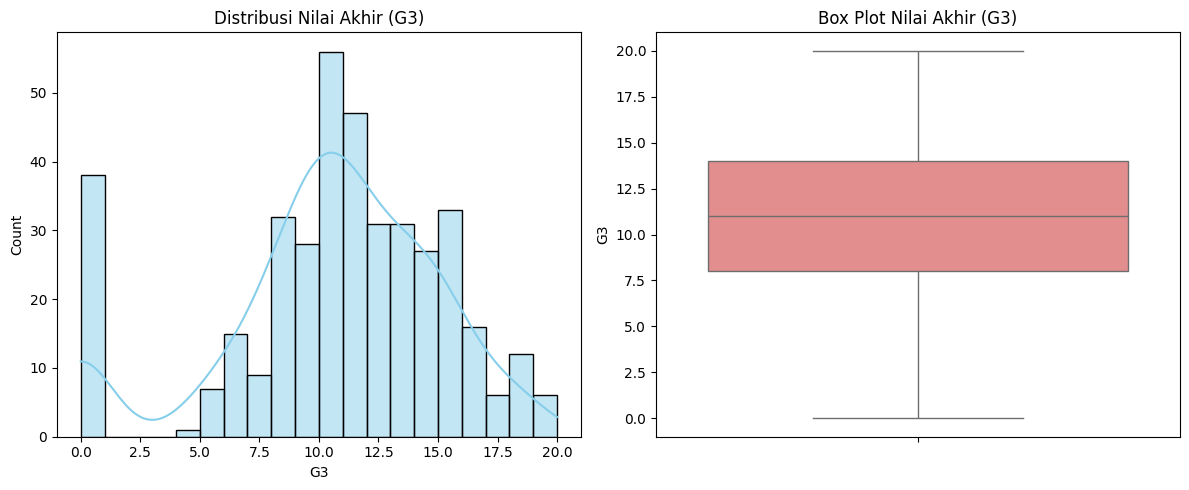
\includegraphics[width=0.8\textwidth]{images/G3Dist.png}
    \caption{Distribusi value G3}
\end{figure}
\begin{figure}[h!]
    \centering
    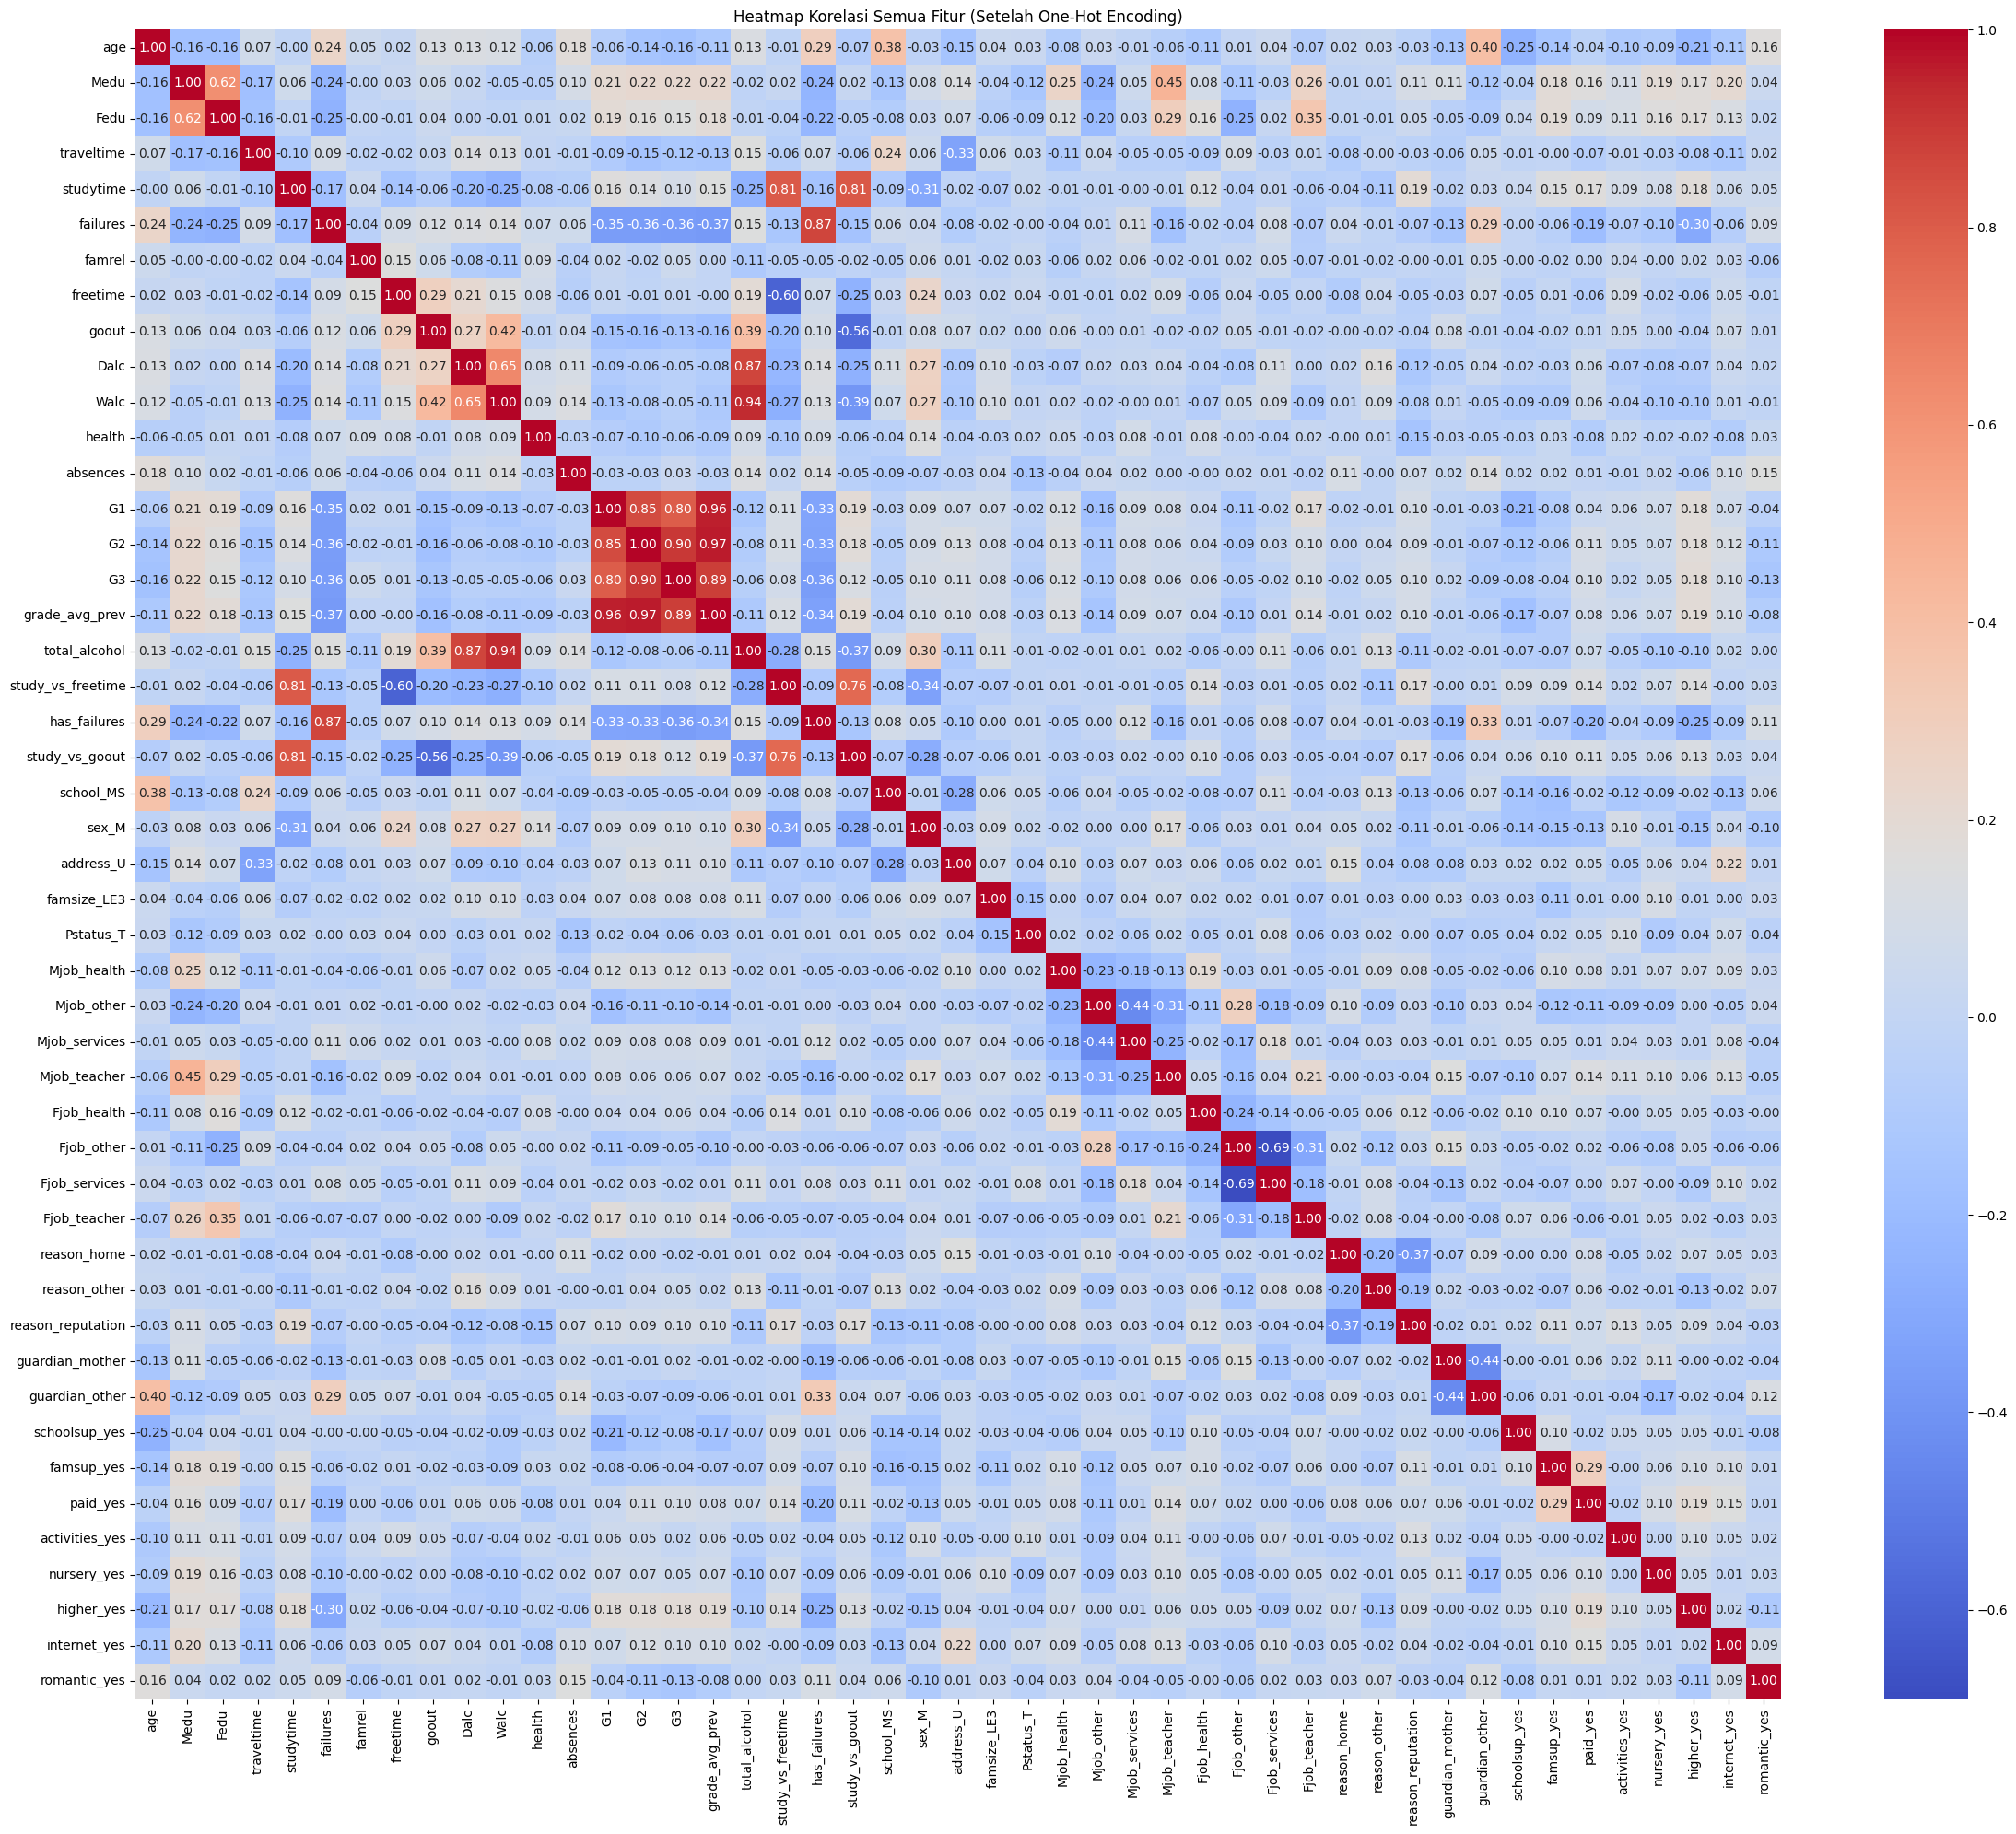
\includegraphics[width=0.8\textwidth]{images/Heatmap.png}
    \caption{Heatmap korelasi antar fitur}
\end{figure}

\subsection{Rekayasa Fitur (Feature Engineering)}
Daripada hanya menggunakan fitur asli, kami membuat fitur-fitur baru yang lebih informatif. Contohnya, \texttt{grade\_avg\_prev} (rata-rata G1 dan G2) dibuat untuk menangkap sinyal kinerja akademik sebelumnya dalam satu variabel kuat. Langkah ini relevan karena seringkali kombinasi fitur memberikan informasi yang lebih berpengaruh daripada fitur individual.
\begin{figure}[h!]
    \centering
    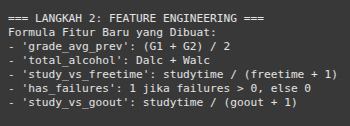
\includegraphics[width=0.8\textwidth]{images/FeatureEng.png}
    \caption{Fitur Baru yang Dibuat dari Data Asli}
\end{figure}

\subsection{One-Hot Encoding}
Model machine learning memerlukan input numerik. Fitur-fitur kategorikal seperti \texttt{sex} (`F'/`M') atau \texttt{higher} (`yes'/`no') diubah menjadi format biner (0 dan 1) melalui One-Hot Encoding. Transformasi ini wajib dilakukan agar algoritma dapat memproses semua informasi yang tersedia dalam dataset.
\begin{figure}[h!]
    \centering
    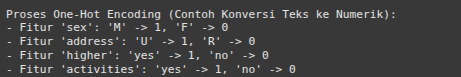
\includegraphics[width=0.8\textwidth]{images/OHE.png}
    \caption{One-Hot Encoding untuk fitur dengan value non-numerik}
\end{figure}

\vspace{0.5cm}
Setelah dataset dipahami dan diproses, fondasi telah siap untuk tahap inti proyek: pembangunan dan evaluasi model-model machine learning.


\chapter*{Metodologi}
\addcontentsline{toc}{chapter}{Hasil Praktikum}

\section{Model Machine Learning yang Digunakan}
Pada proyek ini, digunakan 4 model machine learning berbeda untuk dibandingkan performanya dan dipilih model yang memiliki performa terbaik. Keempat model tersebut adalah regresi linear, random forest, XGboost, dan MLP menggunakan Tensorflow.

\subsection{Regresi Linear}
Regresi linear merupakan salah satu jenis regresi, yaitu metode analisis yang dilakukan untuk mencari hubungan atau korelasi antara dua atau lebih variabel yang memiliki hubungan sebab akibat dan membuat prediksi berdasarkan hubungan tersebut. Pada regresi linear, hubungan antar variabel, yaitu variabel independen dan variabel dependen, memiliki hubungna linear (Kadam, Karhene, dan Mahindrakar. 2020). Dalam konteks machine learning, Regresi linear merupakan algoritma supervised learning yang dapat digunakan untuk melakukan prediksi nilai pada suatu label berdasarkan nilai fitur yang diberikan. Algoritma regresi linear mencari persamaan best-fit line berdasarkan fitur dan label dari dataset yang digunakan untuk training, lalu kemudian menggunakan persamaan best-fit line tersebut untuk melakukan prediksi nilai label apabila diberikan fitur dengan nilai-nilai tertentu. Model machine learning berbasis algoritma regresi linear bekerja dengan baik dalam skenario dataset yang antara fitur dan labelnya memiliki hubungan linear, namun akan memiliki performa yang buruk apabila digunakan untuk melakukan prediksi pada fitur dan label yang memiliki hubungan nonlinear.

\subsection{Random Forest}
Random forest merupakan algoritma ensemble yang bekerja dengan membuat banyak pohon keputusan (decision tree) saat proses training dan memberikan output berupa rata-rata hasil prediksi dari setiap decision tree bila digunakan untuk melakukan prediksi atau hasil mayoritas bila digunakan untuk klasifikasi. Random forest menggabungkan banyak decision tree untuk mengurangi korelasi di antara fitur pada data. Random forest menghilangkan korelasi antar pohon keputusan dengan memilih sampel secara acak dari data training, kemudian dipilih subset fitur secara acak untuk membentuk decision tree. Pengambilan sampel dan fitur secara acak ini mengurangi korelasi antara satu pohon dengan pohon lainnya, sehingga dapat mencegah terjadi overfitting dan bisa mendapatkan akurasi model yang lebih tinggi dibandingkan dengan menggunakan decision tree individual (Salman, Kalakech, dan Steiti. 2024). Pada proyek ini, digunakan model random forest dengan jumlah tree sebanyak 200 unit.

\subsection{XGBoost}
XGBoost (extreme gradient boosting) adalah algoritma ensemble decision tree yang didasarkan pada algoritma gradient boosting, yaitu algoritma yang membangun model secara aditif dengan pertimbangan minimalisasi loss function pada setiap iterasi (Bentéjac, Csörgo, dan Martínez-Muñoz. 2019). XGBoost membentuk decision tree secara sekuensial, dengan decision tree baru memperbaiki atau meningkatkan performa dari iterasi sebelumnya. Layaknya pada gradient boosting yang melakukan minimalisasi loss function untuk setiap iterasi, XGBoost menggunakan algoritma gradient descent untuk meminimalisasi loss function pada setiap pembentukan decision tree baru. Pada proyek ini, digunakan model XGBoost dengan jumlah tree sebanyak 150 unit.

\subsection{Multilayer Perceptron}
Multilayer perceptron (MLP) merupakan jaringan saraf tiruan yang setiap neuronnya menghasilkan jumlah terbobot (weighted sum) dari input neuron tersebut dan ditambahkan dengan sebuah konstan atau bias. Hasil dari proses tersebut kemudian dimasukkan ke dalam fungsi nonlinear yang disebut fungsi aktivasi (Almeida. 2020). MLP memiliki 3 komponen lapisan atau layer neuron, yaitu input layer, hidden layers, dan output layer. Input layer merupakan lapisan neuron yang menerima input berupa fitur-fitur asli yang dimiliki oleh dataset. Hidden layer merupakan lapisan yang bisa terdiri dari satu atau lebih lapisan dan menerima input dari lapisan-lapisan neuron sebelumnya. Output layer merupakan lapisan terakhir dalam jaringan saraf dan hasil dari lapisan ini adalah hasil prediksi model. Pada proyek ini, digunakan model MLP dengan 4 layer, dengan masing-masing layer (diurutkan dari input layer, hidden layer, dan output layer) memiliki 128, 64, 32, dan 1 neuron dan masing-masing neuron menggunakan fungsi aktivasi ReLU (rectified linear unit).

\section{Feature Engineering}
Pada proyek ini, dilakukan feature engineering atau rekayasa fitur untuk memperkaya informasi data pada dataset dengan tujuan meningkatkan performa model. Feature engineering didasarkan pada nilai-nilai yang memiliki korelasi kuat terhadap perubahan nilai G3, misalnya seperti nilai G1 dan G2 yang masing-masing memiliki korelasi sebesar 0,80 dan 0,90 dengan G3. Berdasarkan heatmap korelasi, nilai-nilai ini secara individual memiliki korelasi yang sangat tinggi terhadap nilai G3 dengan hubungan berbanding lurus (semakin tinggi G1 dan G2 semakin tinggi nilai G3). Kedua fitur ini dapat digabungkan untuk membuat fitur baru bernama grade\_avg\_prev, yang merupakan rata-rata nilai dari G1 dan G2, dan setelah ditambahkan ditemukan bahwa fitur baru ini juga memiliki korelasi yang tinggi dengan nilai G3, yaitu sebesar 0,89. Penambahan fitur baru melalui feature engineering membuat dataset menjadi lebih informatif, sehingga dapat meningkatkan performa dari model yang dilatih.

Melalui feature engineering berdasarkan data yang dimiliki dataset, didapatkan 5 fitur baru yang dapat digunakan oleh model, yaitu grade\_avg\_prev, total\_alcohol, study\_vs\_freetime, has\_failures, dan study\_vs\_goout. Fitur grade\_avg\_prev merupakan rata-rata dari nilai G1 dan G2. Fitur total\_alcohol merupakan total konsumsi alkohol dalam satu minggu, didapatkan dari penjumlahan nilai dalc (konsumsi alkohol di hari kerja) dan walc (konsumsi alkohol di akhir pekan). Fitur study\_vs\_freetime merupakan rasio perbandingan antara waktu belajar dan waktu senggang (keduanya dalam jam). Fitur has\_failures merupakan fitur boolean yang menyatakan bahwa siswa pernah memiliki kegagalan sebelumnya. Fitur study\_vs\_goout merupakan rasio perbandingan antara waktu belajar dengan waktu berkegiatan dan bersosialisasi di luar rumah (keduanya dalam jam).

\section{Pemilihan Model}
Pada proyek ini, digunakan 4 model machine learning yang berbeda. Keempat model ini dipilih untuk dibandingkan performanya satu sama lain untuk menemukan dengan dataset, fitur, dan label yang telah ditentukan dalam skenario proyek ini model manakah yang memiliki performa terbaik. Regresi linear dipilih sebagai baseline atau pembanding dasar, hal ini dilakukan karena regresi linear merupakan algoritma model prediktif yang paling sederhana namun memiliki potensi untuk menghasilkan prediksi yang akurat apabila diberikan training menggunakan dataset yang tepat dan digunakan dalam skenario di mana hubungan fitur dengan label sangat linear. Random forest dipilih karena random forest memiliki performa yang baik pada dataset dengan dimensionalitas tinggi, seperti dataset yang digunakan dalam proyek ini yang total memiliki 33 fitur berbeda. XGBoost dipilih karena performanya yang digadang-gadang dapat melampaui random forest, sehingga dapat menjadi pembanding bagi random forest. Multilayer perceptron (MLP) dipilih karena keserbagunaannya yang dapat digunakan di berbagai kasus, salah satunya kasus prediksi nilai. MLP juga bisa memodelkan hubungan nonlinear antara fitur dan label dengan baik, sehingga dapat dijadikan pembanding dengan regresi linear yang merupakan model yang berorientasi pada hubungan linear.


\chapter*{Hasil}
\addcontentsline{toc}{chapter}{Hasil}

Kami melakukan uji coba model dengan skenario dataset yang memiliki total 33 fitur, tidak semua fitur dipakai untuk memprediksi kinerja akademik siswa, kami hanya
memakai 19 fitur. Fitur-fitur yang dipakai 
meliputi nilai ujian sebelumnya {(G1, G2, dan rata-ratanya)}, data demografi dan keluarga {(usia, pendidikan orang tua, jenis kelamin, alamat)}, 
serta kebiasaan belajar dan sekolah (waktu belajar, kegagalan sebelumnya, absensi, akses internet, partisipasi kegiatan). Kami juga menyertakan 
aspek gaya hidup dan sosial siswa, seperti frekuensi bersosialisasi, status kesehatan, status hubungan romantis, dan konsumsi alkohol, dengan jumlah
siswa total 395. Untuk Model Linear Regression yang menggunakan fitur baseline hanya menggunakan fitur absences(Total tidak mengikuti kelas ), 
dan study time.\\

Setelah melakukan uji coba didapatkan hasil sebagai berikut

\section{Uji Coba dengan Data Siswa}

\begin{figure}[h]
    \centering
    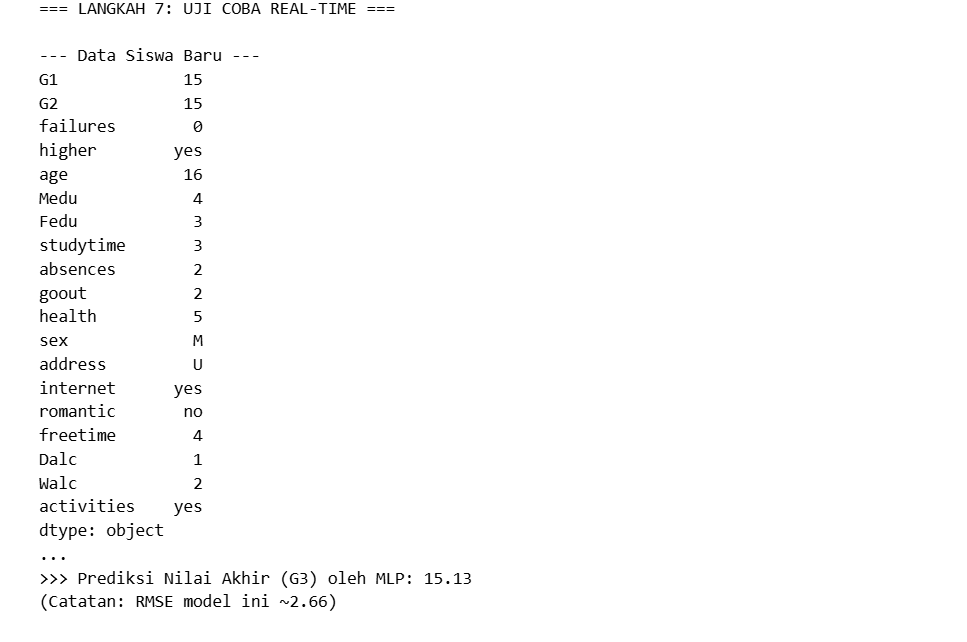
\includegraphics[width=0.8\textwidth]{images/datasiswa2.png}
    \caption{Data Siswa Pertama}
    \label{fig:datasiswa1}
\end{figure}

Di sini pada nilai aktualnya nilai G3 siswa adalah 15, dan saat dilakukan uji coba prediksi didapatkan setiap model seperti yang ada 
pada gambar berikut.

\begin{figure}[h]
    \centering
    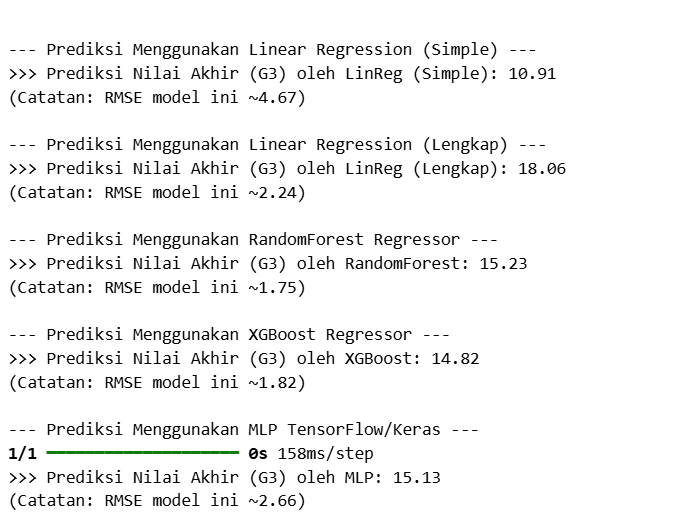
\includegraphics[width=0.8\textwidth]{images/hasil2.png}
    \caption{Hasil Uji Coba Model Pertama}
    \label{fig:hasil1}
\end{figure}

Dilanjutkan uji coba dengan data siswa sebagai berikut:

\begin{figure}[h]
    \centering
    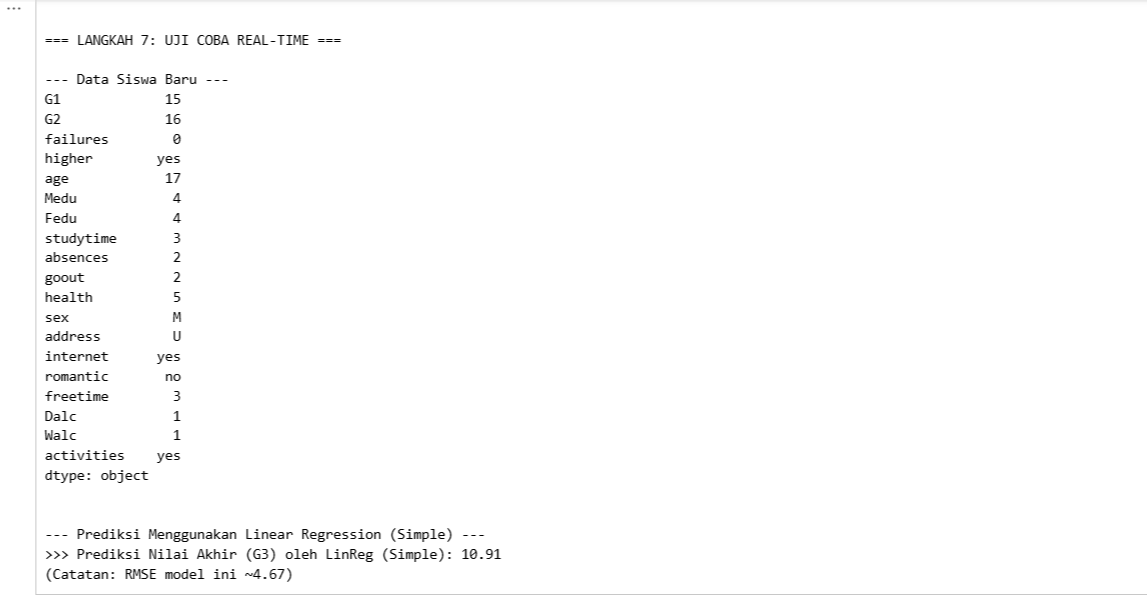
\includegraphics[width=0.8\textwidth]{images/datasiswa1.png}
    \caption{Data Siswa Kedua}
    \label{fig:datasiswa2}
\end{figure}

Dengan data siswa tersebut, kami mengasumsikan bahwa siswa tersebut memiliki nilai G3 sebesar 14,5 yang didapat dengan perkiraan secara 
intuitif menggunakan heatmap yang ada dan didapatkan hasil seperti pada gambar berikut.

\begin{figure}[h]
    \centering
    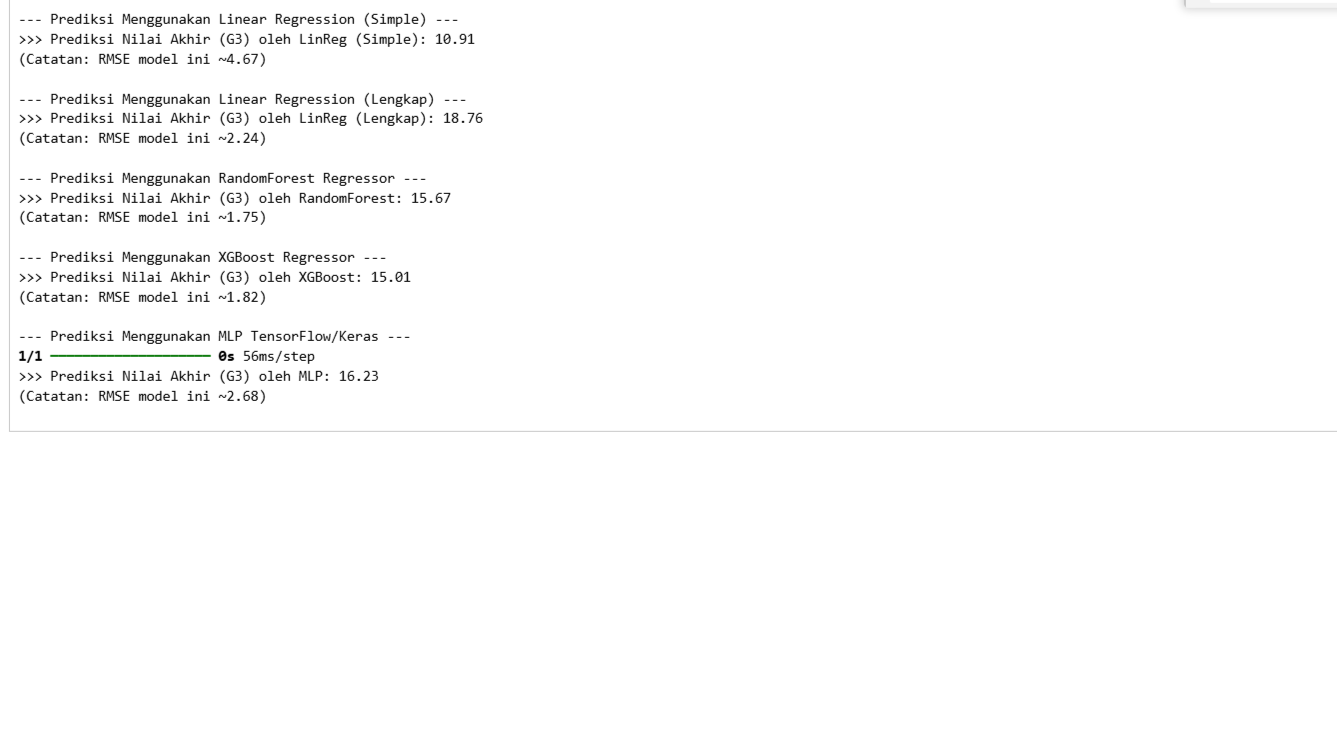
\includegraphics[width=0.8\textwidth]{images/hasil1.png}
    \caption{Hasil Uji Coba Model Kedua}
    \label{fig:hasil2}
\end{figure}

\section{Evaluasi Model}

Berikut adalah visualisasi untuk RMSE (Root Mean Square Error) dan R-Squared, di mana nilai RMSE yang baik adalah mendekati 0 dan R-Squared 
mendekati 1.

\begin{figure}[h]
    \centering
    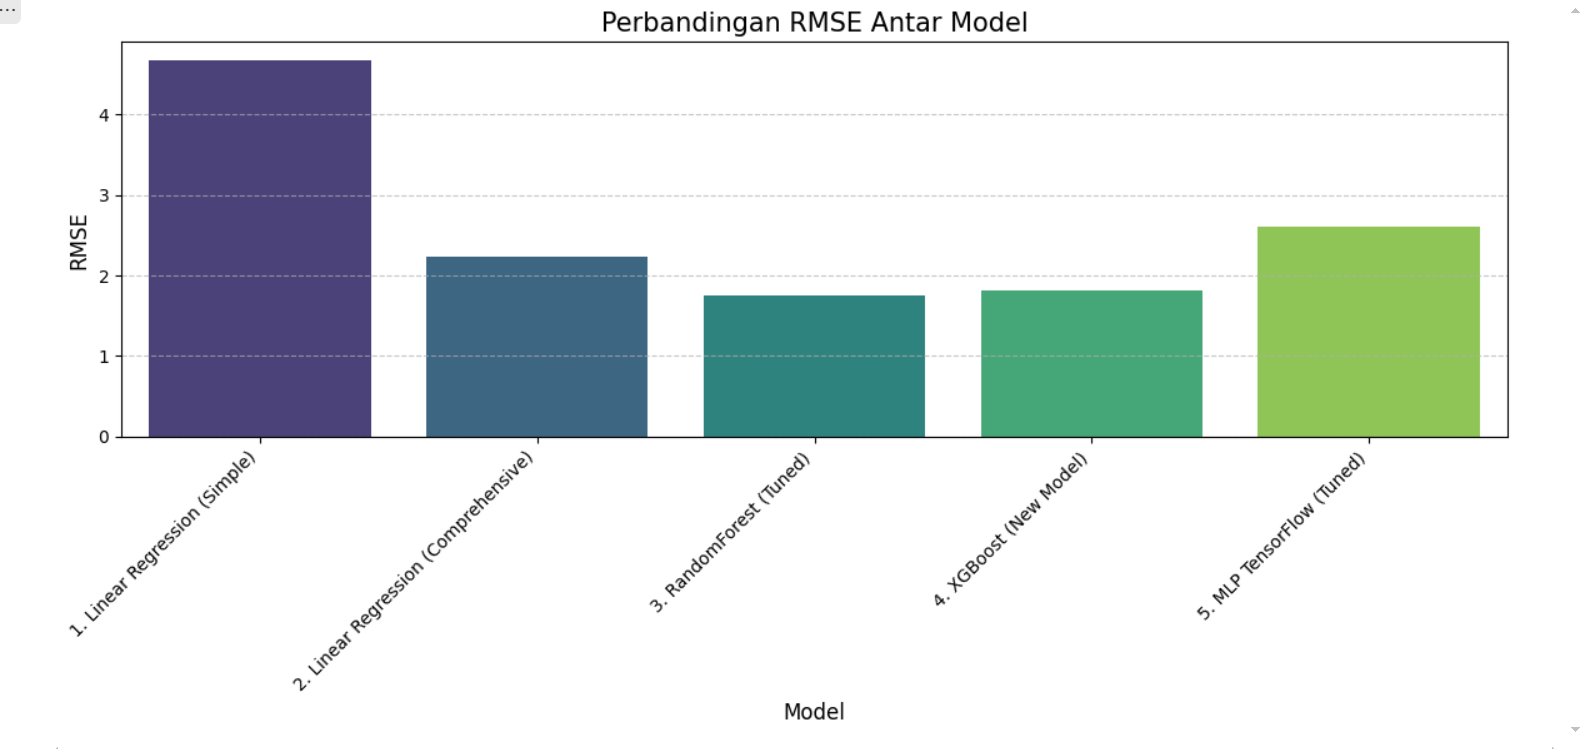
\includegraphics[width=0.8\textwidth]{images/rmse.png}
    \caption{Visualisasi RMSE}
    \label{fig:rmse}
\end{figure}

\begin{figure}[h]
    \centering
    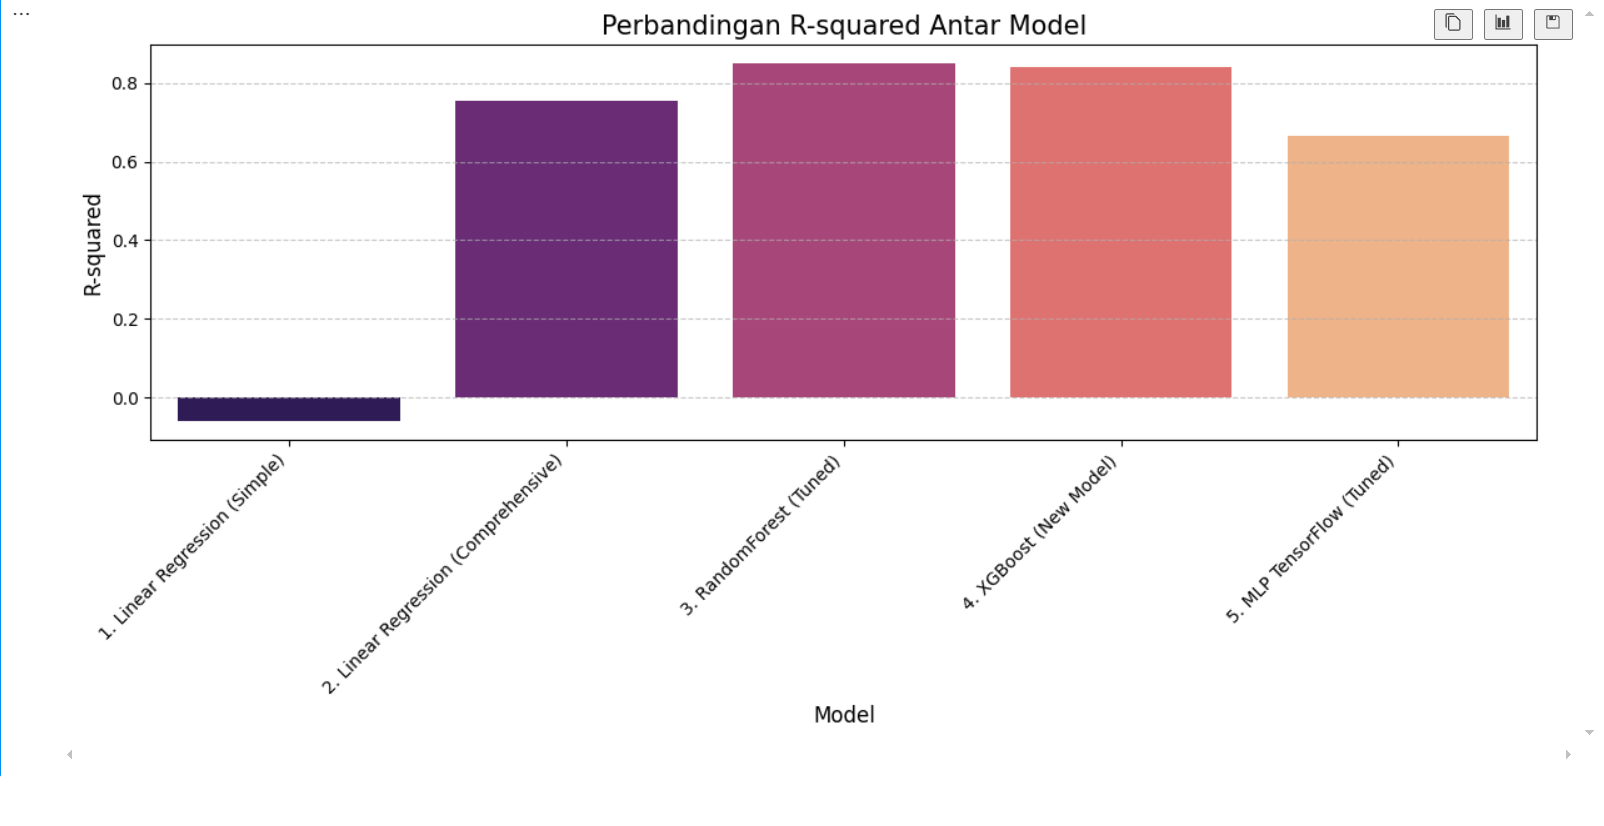
\includegraphics[width=0.8\textwidth]{images/r-squared.png}
    \caption{Visualisasi R-Squared}
    \label{fig:rsquared}
\end{figure}

Dari data tersebut RandomForest Regressor mendapatkan nilai RMSE yang lebih rendah daripada semua model yang ada, diikuti oleh XGBoost, 
Linear Regression dengan fitur yang lengkap, lalu MLP TensorFlow. Nilai RMSE menunjukkan berapa rentang error yang dihasilkan oleh data. 
Untuk R-Squared, RandomForest Regressor juga merupakan yang paling baik di antara model yang ada. R-Squared menunjukkan informasi mengenai 
bagaimana model tersebut menjelaskan variabilitas data terhadap model yang digunakan. R-Squared menggambarkan seberapa baik model sesuai 
dengan data yang digunakan. Secara teknis, RandomForest Regressor mungkin lebih cocok untuk dataset yang relatif lebih kecil dibandingkan
MLP TensorFlow dan XGBoost.RandomForest kami anggap lebih tidak rumit dalam interpretasi dan implementasi dibandingkan dua model lainnya.\\

Dapat dilihat bahwa performa model RandomForest Regressor adalah model dengan prediksi yang paling akurat dibandingkan dengan model-model lain. 
Hal ini dapat terjadi dikarenakan RandomForest Regressor merupakan model yang memang cocok untuk dataset yang lebih kecil daripada menggunakan MLP TensorFlow 
dan XGBoost. Jika dibandingkan secara teknis, RandomForest merupakan model yang paling tidak rumit dibanding dua model tersebut. RandomForest 
Regressor bekerja dengan membuat decision tree secara paralel dengan memilih data secara acak, dan dari decision tree yang sudah dibuat secara 
paralel nilai prediksi dari setiap decision tree tersebut akan dirata-rata untuk mendapatkan hasilnya. XGBoost juga masih menggunakan decision 
tree, namun dengan cara memperbaiki kesalahan berulang kali dari decision tree sebelumnya. Untuk penjelasan simpelnya, MLP TensorFlow sendiri 
merupakan salah satu model jaringan saraf tiruan yang memiliki tiga komponen, yaitu \textit{Input Layer}, \textit{Hidden Layer}, 
dan \textit{Output Layer} yang memiliki cara pemodelan yang lebih kompleks dibandingkan RandomForest Regressor dan XGBoost.

\section{Visualisasi Scatter Plot}

Kami juga melakukan visualisasi menggunakan scatter plot.

\begin{figure}[h]
    \centering
    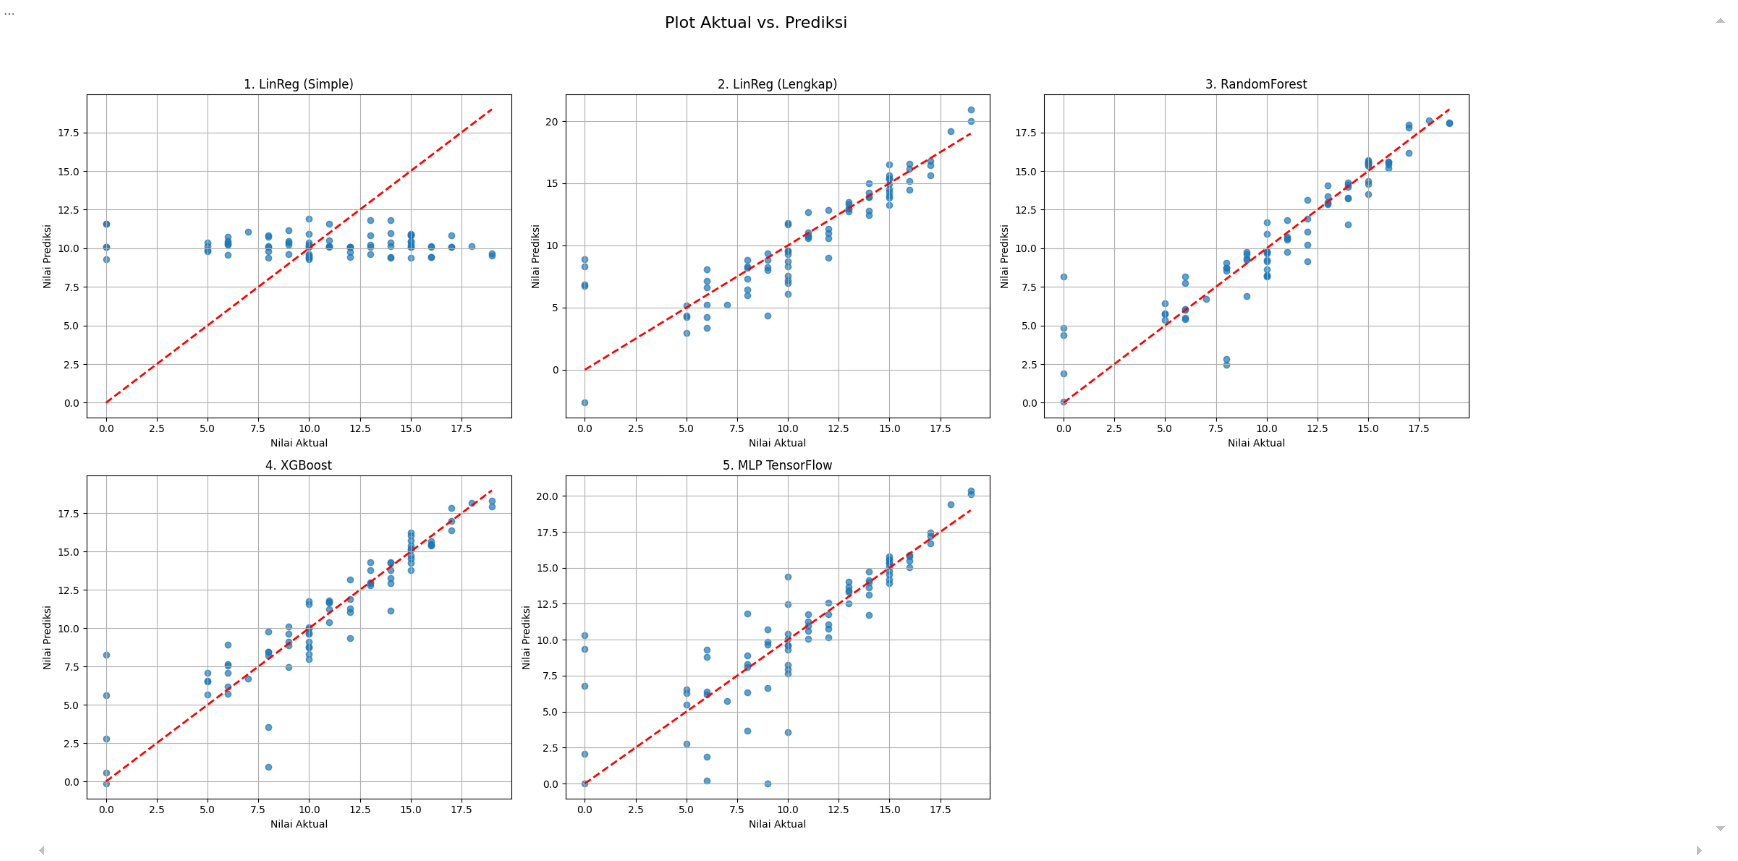
\includegraphics[width=0.8\textwidth]{images/scatter_plot.png}
    \caption{Visualisasi Scatter Plot}
    \label{fig:scatter}
\end{figure}

Dari visualisasi scatter plot yang membandingkan nilai aktual dengan nilai prediksi untuk setiap model, beberapa wawasan penting dapat ditarik 
mengenai performa dan karakteristik setiap algoritma. Idealnya, titik-titik pada scatter plot harus terkonsentrasi rapat di sepanjang garis 
diagonal merah (y=x), menunjukkan bahwa nilai prediksi sangat mendekati nilai aktual.\\

Model RandomForest Regressor dan XGBoost menunjukkan performa yang paling baik dalam visualisasi ini. Titik-titik data untuk kedua model ini 
tampak paling padat dan terpusat di sekitar garis diagonal. Ini mengindikasikan bahwa baik RandomForest maupun XGBoost mampu menangkap hubungan 
kompleks dalam data dan menghasilkan prediksi yang konsisten dan akurat di berbagai rentang nilai G3. Kerapatan titik di sekitar garis 
menunjukkan bahwa error prediksi (perbedaan antara aktual dan prediksi) cenderung kecil dan terdistribusi merata.\\

Sebaliknya, model Linear Regression yang menggunakan fitur baseline menunjukkan sebaran titik yang lebih luas dan menyebar jauh dari garis 
diagonal. Ini terutama terlihat pada nilai-nilai G3 yang lebih ekstrem (sangat rendah atau sangat tinggi), di mana prediksi cenderung 
menyimpang lebih jauh dari nilai aktual. Sebaran yang lebih tersebar tidak merata mencerminkan keterbatasan model linear dalam menangkap 
hubungan non-linear atau interaksi kompleks antar fitur, yang mengakibatkan nilai RMSE yang lebih tinggi dibandingkan model berbasis pohon dan MLP TensorFlow   .\\

Model MLP TensorFlow menunjukkan performa yang kurang baik, berada setelah Linear Regression yang menggunakan fitur lengka dan RandomForest/XGBoost. Meskipun titik-titiknya tidak 
sepadat RandomForest atau XGBoost, mereka tetap menunjukkan konsentrasi yang baik di sekitar garis diagonal. Ini menegaskan bahwa MLP adalah 
model yang efektif dan mampu memberikan prediksi yang cukup akurat, meskipun dalam kasus ini RandomForest sedikit unggul.\\

Secara keseluruhan, scatter plot ini secara visual mengkonfirmasi metrik evaluasi yang disajikan sebelumnya. Model-model yang memiliki nilai 
R-Squared tinggi dan RMSE rendah (seperti RandomForest dan XGBoost) ditunjukkan dengan titik-titik yang sangat dekat dengan garis ideal, 
sementara model dengan metrik yang kurang baik menunjukkan sebaran yang lebih lebar. Visualisasi ini juga membantu mengidentifikasi rentang 
nilai di mana suatu model mungkin berkinerja kurang baik atau di mana terdapat outlier prediksi.



\chapter*{Diskusi}
\addcontentsline{toc}{chapter}{Diskusi}


Saat kami hanya menggunakan beberapa fitur, nilai prediksi sangatlah tidak akurat, baru setelah kami menggunakan fitur yang lebih banyak dan mempunyai pengaruh pada nilai G3 dan membuat fitur 
baru dari beberapa fitur nilai prediksi menjadi akurat, hal ini dapat terlihat pada hasil prediksi menggunakan model linear regressi yang menggunakan
fitur baseline dan fitur yang lengkap perbedaan keakuratan nilai prediksi sangatlah jauh, sehingga kami menyadari bahwa menggunakan fitur yang berkaitan 
dengan nilai yang ingin dicari sangat penting untuk mencapai nilai prediksi model yang baik\\

Hasil yang diperoleh dari uji model menggunakan dataset ini adalah model RandomForest Regressor yang terbaik pada skenario ini yaitu dataset 
yang memiliki banyak fitur namun jumlah data yang ada pada dataset hanya 395 dimana data ini relatif cukup kecil jika dibandingkan dengan lainnya.
Pada dataset kami, kami memiliki keterbatasan untuk menguji model ini pada dataset yang lebih banyak sehingga dapat melihat potensial penuh dari 
XGboost,dan MLP TensorFlow. Rekomendasi dari kami penulis adalah untuk mencoba model ini pada dataset yang mempunyai data yang lebih banyak daripada 
dataset ini untuk mendapatkan potensi penuh dari XGboost,dan MLP TensorFlow.


\chapter*{Kesimpulan}
\addcontentsline{toc}{chapter}{Kesimpulan}

%Isi dengan Kesimpulan Praktikum

\lipsum[6-7] %Hapus jika ada kesimpulan praktikum

\end{document}
